\chapter{Rapportens struktur} \label{metode}
Denne rapport tager udgangspunkt i metoden for en MTV, hvor en medicinsk problemstilling analyseres \citep{mtvhaandbog}. Yderligere er rapporten udarbejdet som et semesterprojekt på Aalborg Universitet, hvorfor den også tager udgangspunkt i problembaseret læring, hvor der opstilles et initierende problem, laves en problemanalyse og en problemformulering, der forsøges at besvare. 

\begin{figure}[H]
	\centering
	\includegraphics[width=0.5\textwidth]{figures/metodemodel}
	\caption{Model for den brugte metode i projektet.}
	\label{fig:metodemodel}
\end{figure}

\noindent
Som illustreret på \autoref{fig:metodemodel}, starter projektet bredt med et initierende problem, som analyseres og afgrænses i en problemformulering. Denne problemformulering forsøges besvaret gennem en MTV. 

En MTV er en vurdering baseret på forskning og kan herved anvendes som et evidensbaseret grundlag, når der skal tages beslutninger om, hvorvidt nye teknologier bør anvendes i sundhedsvæsenet. Målgruppen for en MTV er beslutningstagere, såsom politikere, ledelser på sygehuse og organisationer. De fire hovedområder indenfor MTVen; teknologi, patient, organisation og økonomi, kræver forskellige metoder, videnskabelige teorier, forskingstilgange med mere, og på baggrund af dette er der ofte fagfolk fra relevante områder involveret i udarbejdelsen af en MTV \citep{mtvhaandbog}. 

MTV-analyserne belyser forskellige aspekter af teknologien ved at inddele MTV'en i fire områder; teknologi, patient, organisation og økonomi. 

Hvert aspekt har et tilhørende metodeafsnit til at beskrive, hvilke analysemetoder og MTV-spørgsmål, der anvendes, og som er relevante for at kunne besvare den opstillede problemformulering. Informationen er primært fundet gennem systematiske informationssøgninger og er tilpasset, med henblik på besvarelse af MTV-spørgsmålene i de fire aspekter. Metoden for informationssøgning beskrives yderligere i \autoref{sec:metode_soeg}. Ud over en systematisk informationssøgning indsamles information ud fra egne erfaringer om teknologien, hvilke kan være relevante for besvarelsen af visse MTV-aspekter. Disse erfaringer ses især relevante for de områder, hvor den eksisterende viden ikke har været tilstrækkelig for at kunne besvare de fokuserede spørgsmål under MTV-analyserne.

I syntesen vil de fire MTV-områder blive diskuteret, og der vil være en samlet konklusion på problemformuleringen ud fra delkonklusionerne i de fire MTV-analyser. 


Idet denne MTV-inspirerede rapport er udarbejdet af en sundhedsteknologi projektgruppe på 5. semester, anses det, at rapporten kan anvendes som vidensgrundlag til en beslutningstagen eller til videre undersøgelser. 


\chapter{MTV-analyse}
Følgende kapitel beskriver de anvendte metoder i henholdsvis teknologi-, patient-, organisations- og økonomianalysen. Endvidere vil MTV-spørgsmålene til hver analyse fremgå. 

\section{Teknologi}\label{sec:metode_tek}
Teknologiafsnittet er skrevet ud fra MTV-spørgsmål, som vil beskrive teknologien og redegøre for og vurdere, hvilke teknologiske krav, Fitbit Flex skal opfylde for at kunne benyttes til at måle aktivitetsniveau hos hypertensive patienter. 
Foruden en tilpasset litteratursøgning, foretages beskrivelse af teknologien ud fra erfaringer ved anvendelse af software, der er relateret til teknologien \citep{mtvhaandbog}. Dette giver anledning til følgende MTV-spørgsmål: 
\subsection{MTV-spørgsmål}
\begin{itemize}
\item Hvordan fungerer Fitbit Flex, og hvordan kan dette anvendes, således at en alment praktiserende læge får dokumenteret patientens aktivitetsniveau?
\item Repræsenterer Fitbit Flex den fysiske aktivitet tilstrækkeligt, til at data kan anvendes af praktiserende læger til vurdering af patientens fysiske aktivitetsniveau?
\end{itemize}

\section{Patient}\label{sec:metode_pat}
Til analyse af patientaspektet, og hvordan teknologien påvirker denne, analyseres sociale, kommunikative, økonomiske, individuelle og etiske forhold, samt samspillet mellem disse. Dette gøres ud fra metoden for en MTV \citep{mtvhaandbog}.

\begin{figure}[H]
\centering
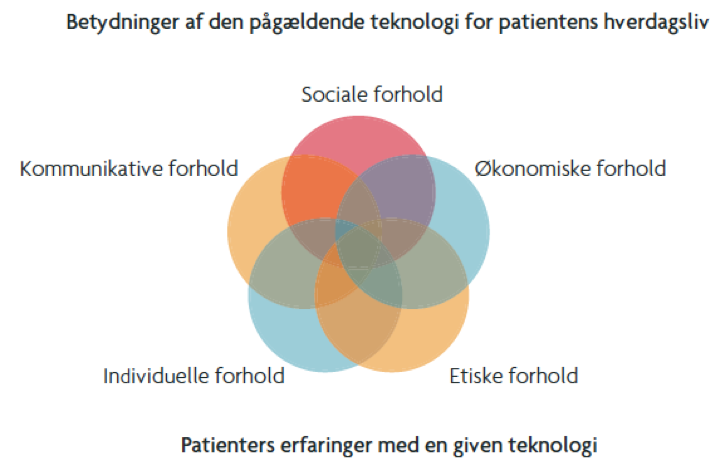
\includegraphics[width=0.8\textwidth]{figures/patientaspekter}
\caption{Fokusområder for patientanalysen. Cirklerne repræsenterer henholdsvis de sociale, økonomiske, etiske, individuelle og kommunikative forhold, og overlappene illustrerer samspillet derimellem \citep{mtvhaandbog}.}
\label{fig:patientaspekter}
\end{figure}

\noindent
Figur \ref{fig:patientaspekter} viser de forskellige forhold for patientaspektet, der tages højde for i analysen \citep{mtvhaandbog}. I forhold til Fitbit Flex fokuseres der i denne analyse på sociale forhold, herunder hvordan denne teknologi påvirker patientens arbejds- og uddannelsesliv, familie og livskvalitet, individuelle forhold, herunder hvordan patienten oplever teknologien, kommunikative forhold, samt etiske forhold, herunder risiko for misbrug af personlige data. Dette giver anledning til følgende MTV-spørgsmål: 

\subsection{MTV-spørgsmål}
\begin{itemize}
\item Hvilke kriterier skal være opfyldt for, at patienten kan få udleveret Fitbit Flex?
\item Er teknologien brugervenlig og motiverer den patienten til at få en mere aktiv hverdag?
\item Hvordan påvirker teknologien patienternes individuelle og sociale forhold i dagligdagen?
\item Hvor stor en andel af patienter oplever en positiv virkning ved anvendelse af teknologien, hvad er tidshorisonten for denne virkning, og hvad spiller en rolle for, at teknologien giver et succesfuldt forløb?
\item Hvilke etiske dilemmaer opstår ved at monitorere patientens fysiske aktivitet?
\end{itemize} 

\section{Organisation}\label{sec:metode_org}
Det ønskes at undersøge de organisatoriske forudsætninger samt mulige konsekvenser ved implementering af Fitbit Flex til monitorering af fysisk aktivitet i almen praksis. Undersøgelsen tager udgangspunkt i den modificerede Leavitt organisationsmodel der ses af \autoref{fig:leavittmodel}, for at analysere konsekvenserne af en eventuel ændring i organisationen \citep{mtvhaandbog}. 

\begin{figure}[H]
\centering
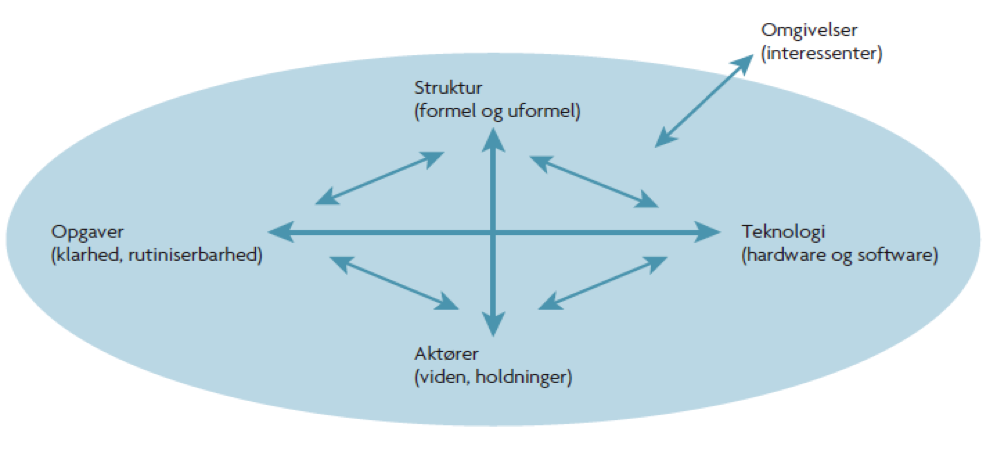
\includegraphics[width=0.9\textwidth]{figures/leavitt}
\caption{Leavitts modificerede organisationsmodel. Pilen mellem de forskellige områder betegner sammenspillet mellem dem. Dertil står omgivelser uden for de andre fire områder, da dette betegner, hvem der har interesse for de organisatoriske ændringer, der vil forekomme \citep{mtvhaandbog}.}
\label{fig:leavittmodel}
\end{figure}

\noindent
Leavitts modificerede organisationsmodel benyttes, da denne tager højde for omgivelsernes påvirkning på teknologi, aktører, opgaver, struktur, disses indbyrdes påvirkning og påvirkning på omgivelserne. 
Teknologi omhandler arbejdsprocesser, procedurer og rutiner, i relation til teknologien.  
Aktører er de ansatte i organisationen, og deres holdninger og ekspertise i relation til organisationens opgaveløsninger. 
Opgaver dækker over karakteren af de opgaver, som organisationen forsøger at løse. 
Struktur omhandler formelle mønstre i organisationen, som arbejdsdeling og formalisering.  
Omgivelser er udvalgte interessenter, der er relevante i forhold til de organisatoriske ændringer \citep{mtvhaandbog}. Dette giver anledning til følgende MTV-spørgsmål:

\subsection{MTV-spørgsmål}
\begin{itemize}
\item Hvordan passer Fitbit Flex i almen praksis? 
\item Hvilke krav vil implementeringen stille til alment praktiserende læger, og hvem skal stå for en eventuel efteruddannelse? 
\item  Hvordan vil patientfordelingen mellem den primære og sekundære sundhedssektor blive påvirket, og hvad vil en ændring i arbejdsfordelingen medføre?
\end{itemize}

\section{Økonomi}\label{sec:metode_oeko}
I økonomianalysen undersøges mulige omkostninger ved implementering og anvendelse af Fitbit Flex som monitoreringsenhed for fysisk aktivitet til brug i almen praksis.
Ligeledes undersøges omkostninger for den nuværende monitoreringsmetode, samt hvilke økonomiske konsekvenser, der forekommer, når patienten ikke dyrker den anbefalede mængde motion.
Det ønskes at foretage cost-effectiveness og cost-utility analyser for at afgøre, om Fitbit Flex skal implementeres. I en cost-effectiveness analyse opgøres omkostninger og konsekvenser ved den nuværende monitoreringsmetode og Fitbit Flex for at afgøre, hvilken teknologi der er mest omkostningseffektiv i forhold til både valuta og antal vundne leveår. En cost-utility analyse benyttes til at tage højde for kvalitetsjusterede leveår (QALY), hvor de vundne leveår kvalitetsjusteres med den helbredsrelaterede livskvalitet \citep{mtvhaandbog}.
I denne økonomianalyse vil blive fremhævet mulige sundhedsmæssige resultater som følge af implementeringen af Fitbit Flex, i forhold til udgifterne dertil, uden at foretage egentlige cost-effectiveness eller cost-utility analyser, eftersom de benyttede værdier i analysen er estimerede.  
Disse estimerede værdier er baseret på udregninger ud fra funden litteratur omkring sundhedsøkonomi. Dette giver anledning til følgende MTV-spørgsmål: 

\subsection{MTV-spørgsmål}
 
\begin{itemize}
\item Hvad er omkostningerne ved nuværende monitoreringsmetode, samt konsekvenserne ved utilstrækkelig aktivitetsydelse? 
\item Hvilke omkostninger er forbundet med brug af Fitbit Flex til patienter med hypertension, og hvad er den økonomiske konsekvens af dette, hvis brug af aktivitetsarmbånd resulterer i et øget antal kvalitetsjusterede leveår?
\end{itemize}


%  Søgeprotokollen findes i \autoref{app:soegeprotokol}.